\begin{example}
    Ряд Лорана может не иметь кольца сходимости вовсе. Например, \(\sum\limits_{n = -\infty}^
    {+\infty} z^n\).
\end{example}

Заметим, что ряд \(N_2\) сходится локально равномерно в \(|z-z_0| < r\). Обоснуем почему ряд
\(N_1\) сходится локально равномерно в \(|z-z_0| > \dfrac{1}{\rho}\). Ряд \((**)\) сходится локально
равномерно в круге \(|w| < \rho\) из теоремы Абеля. Пусть \(E\)~--- произвольный компакт, который 
содержится в \(|z-z_0| > \dfrac{1}{\rho}\). Образ \(E\) при непрерывном отображении \(\dfrac{1}
{z-z_0}\) есть компакт \(D \subset \{|w|<\delta\}\). На \(D\) ряд \((**)\) сходится равномерно
в следствие теоремы Абеля, а значит ряд \(N_1\) сходится равномерно на \(E\). Вследствие 
произвольности \(E\) доказана локальная равномерная сходимость \(N_1\) в \(|z-z_0| > \dfrac{1}
{\rho}\). Из этих фактов, а также 1 и 2 теорем Вейерштрасса следует доказательство следующего
утверждения:

\begin{statement}
    Верно следующее:
    \begin{enumerate}[wide=20pt, label=\arabic*., itemsep=0ex]
        \item В кольце сходимости \(K\) сумма ряда \((*)\)~--- регулярная функция;
        \item Сумму ряда Лорана в этом кольце можно почленно дифференцировать.
    \end{enumerate}
\end{statement}

\begin{statement}
    Пусть \(f(z)\) регулярна в \(K\colon \, 0 \le R_1 < |z-z_0|< R_2 \le +\infty\). Тогда в \(K\)
    существует и единственно разложение в ряд Лорана \(f(z) = \sum\limits_{n = -\infty}^{-1} c_n 
    (z-z_0)^n + \sum\limits_{n=0}^{\infty} c_n (z-z_0)^n\) и \[c_n = \dfrac{1}{2 \pi i} 
    \int\limits_{|z - z_0| = \rho \in (R_1, R_2)} \dfrac{f(\zeta) d\zeta}{(\zeta - z_0) ^ {n+1}}, \,
    n \in \Z \tag{3}\].
\end{statement}

\begin{proof}
    Пусть \(z \in K\) фиксировано. Выберем и зафиксируем \(r_1, r_2\) такие, что \(R_1 < r_1 < 
    |z-z_0| < r_2 < R_2\). 
    
    \noindent
    \begin{minipage}[c]{0.3\textwidth}
        \centering
        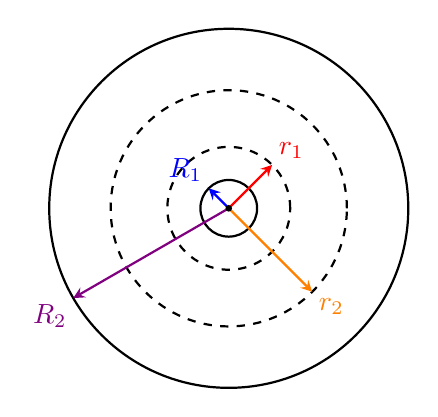
\begin{tikzpicture}[scale=0.6] % Масштаб можно регулировать, чтобы картинка не была слишком большой
            % Центр окружностей
            \coordinate (O) at (0,0);

            % 2. Окружности
            \draw[thick] (O) circle (0.6);         % Самая маленькая (сплошная)
            \draw[dashed, thick] (O) circle (1.3); % Вторая (штриховая)
            \draw[dashed, thick] (O) circle (2.5); % Третья (штриховая)
            \draw[thick] (O) circle (3.8);         % Самая большая (сплошная)

            % 3. Стрелки радиусов в порядке возрастания

            % R_1 (угол 135 градусов)
            \draw[->, >=stealth, blue, thick] (O) -- (135:0.6) 
                node[anchor=south east, inner sep=2pt] {$R_1$};

            % r_1 (угол 45 градусов)
            \draw[->, >=stealth, red, thick] (O) -- (45:1.3) 
                node[anchor=south west, inner sep=2pt] {$r_1$};

            % r_2 (угол -45 градусов)
            \draw[->, >=stealth, orange, thick] (O) -- (-45:2.5) 
                node[anchor=north west, inner sep=2pt] {$r_2$};

            % R_2 (угол 210 градусов)
            \draw[->, >=stealth, violet, thick] (O) -- (210:3.8) 
                node[anchor=north east, inner sep=2pt] {$R_2$};

            % Центральная точка
            \fill (O) circle (2pt);
        \end{tikzpicture}
    \end{minipage}%
    \hfill % Равномерный отступ между левым и правым блоком
    \begin{minipage}[c]{0.67\textwidth}
        По интегральной теореме Коши для \(f(z)\) в ОСПГ \(D = \{|z-z_0| \in (r_1, r_2)\}\) имеем:
        \[
        f(z) = \dfrac{1}{2 \pi i} \int\limits_{|z-z_0| = r_2} \dfrac{f(\zeta) d\zeta}{\zeta - z_0} -
        \dfrac{1}{2 \pi i} \int\limits_{|z-z_0| = r_1} \dfrac{f(\zeta) d\zeta}{\zeta - z_0} = N_1 + 
        N_2. \tag{4}
        \]

        \(N_2\)~--- интеграл Коши. Так как кргу \(|\zeta - z_0| < r_2\) не пересекается с 
        окружностью \(|\zeta - z_0| = r_2\), то по утверждению \ref{14:int_koshi} \(N_2 = 
        \sum\limits_{n = 0}^\infty c_n (z-z_0)^n\), где 
        \[
        c_n = \dfrac{1}{2 \pi i} \int\limits_{|z - z_0| = r_2} \dfrac{f(\zeta) d\zeta}{(\zeta - z_0)
         ^ {n+1}}. \tag{5}
        \]
    \end{minipage}

    Рассмотрим \(N_1\). Имеем следующее:
    \[
    - \dfrac{1}{\zeta - z} = \dfrac{1}{z - \zeta} = \dfrac{1}{(z-z_0) - (\zeta - z_0)} = 
    \dfrac{1}{z-z_0} \dfrac{1}{1 - \frac{\zeta - z_0}{\zeta - z_0}} = \sum\limits_{n=0}^{+\infty}
    \dfrac{(\zeta - z_0)^n}{(z - z_0)^{n+1}} \tag{6}
    \]

    Ряд в правой части \((6)\) сходится равномерно на \(|\zeta - z_0| = r_1\) по признаку 
    Вейерштрасса, так как \(\left|\dfrac{r_1}{\zeta - z_0}\right| < 1\). Тогда из \((6)\) следует:
    \[
    - \dfrac{f(\zeta)}{2 \pi i} \dfrac{1}{\zeta - z_0} = \sum\limits_{n=0}^{+\infty} 
    \dfrac{f(\zeta)}{2 \pi i} \dfrac{(\zeta - z_0)^n}{(z - z_0)^{n+1}} \tag{7}
    \]

    Этот ряд сходится равномерно на окружности \(|\zeta - z_0| = r_1\) в силу ограниченности 
    \(f(\zeta)\). Интегрируя \((7)\) почленно имеем:
    \[
    N_1 = \sum\limits_{n=0}^{+\infty} (\dfrac{1}{2 \pi i}\int\limits_{|\zeta - z_0| = r_1} 
    f(\zeta) (\zeta - z_0)^n) (z-z_0)^{-n-1} = \sum\limits_{m = - \infty} ^ {-1} (\dfrac{1}{2 \pi i}
    \int\limits_{|\zeta - z_0| = r_1} \dfrac{f(\zeta) d\zeta}{(\zeta - z_0)^{m+1}}) (z-z_0)^m 
    \tag{8}
    \]

    Итак доказана возможность разложения в ряд Лорана для любого \(z \in \{R_1 < |z-z_0| < R_2\}\).
    Осталось доказать, что в формулах \((5)\) и \((8)\) можно взять любое \(\rho \in (R_1, R_2)\).

    Зафиксируем \(R_1 < \rho_1 < \rho_2 < R_2\) и зафиксируем \(n \in \Z\). Функция \(g(\zeta) = 
    \dfrac{1}{2 \pi i} \dfrac{f(\zeta)}{(\zeta - z_0)^{n+1}}\) регулярна в ОСПГ \(\rho_1 < |\zeta - 
    z_0| < \rho_2\). По интегральной теореме Коши для этой ОСПГ имеем:
    \[
    \int\limits_{|\zeta - z_0| = \rho_1} g(\zeta) d\zeta = \int\limits_{|\zeta - z_0| = \rho_2} 
    g(\zeta) d\zeta
    \]

    Докажем единственность разложения в ряд Лорана. Зафиксируем \(\rho \in (R_1, R_2)\). Тогда 
    \(\int\limits_{|z-z_0| = \rho} \dfrac{dz}{z-z_0} = 2 \pi i\). Пусть в кольце есть 2 разложения
    \(\sum\limits_{n = -\infty}^{+\infty} c_n (z-z_0)^n \equiv \sum\limits_{n = -\infty}^{+\infty} 
    d_n (z-z_0)^n\). Зафиксируем \(m \in \Z\). Тогда \(\sum\limits_{n = -\infty}^{+\infty} c_n 
    (z-z_0)^{m+n} \equiv \sum\limits_{n = -\infty}^{+\infty} d_n (z-z_0)^{m+n}\). Интегрируя по 
    окружности \(|z-z_0| = \rho\) получаем \(\sum\limits_{n = -\infty}^{+\infty} c_n 
    \int\limits_{|z-z_0| = \rho} (z-z_0)^{m+n} dz \equiv \sum\limits_{n = -\infty}^{+\infty} d_n 
    \int\limits_{|z-z_0| = \rho}(z-z_0)^{m+n} dz\). Все интегралы занулятся за исключением \(n+m = 
    -1\), так как при всех остальных \(n\) подынтегральная функция имеет первообразную, а значит
    \(c_{-m-1} \cdot 2 \pi i = d_{-m-1} \cdot 2 \pi i\). В силу произвольности \(m\) получаем
    \(c_n = d_n, \forall n \in \Z\).
\end{proof}

Рассмотрим неравенство Коши для коэффициентов ряда Лорана. Пусть \(\rho \in (R_1, R_2)\) фиксировано
и \(M(\rho) = \max\limits_{|\zeta - z_0| = \rho} |f(\zeta)|\). По формулам об оценке интегралов
получаем следующее:

\[|c_n| = \left|\dfrac{1}{2 \pi i} \int\limits_{|\zeta - z_0| = \rho} \dfrac{f(\zeta) d\zeta}{|\zeta
- z_0|^{n+1}}\right| \le \dfrac{1}{2 \pi} \dfrac{M(\rho)}{\rho^{n+1}} 2\pi \rho = 
\dfrac{M(\rho)}{\rho^{n}}\]


\Section{Изолированные особые точки}

\begin{definition}
    Точка \(z_0 \in \oCo\) называется изолированной особой точкой (ИОТ) для \(f(z)\), если 
    существует \(\mathring{B}_R(z_0)\), что \(f(z)\) регулярна в \(\mathring{B}_R(z_0)\), но не
    регулярна или не определена в \(z_0\).
\end{definition}

Тип ИОТ будем определять по пределу функции \(f(z)\) при \(z \rightarrow z_0\). Если \(\exists 
\lim\limits_{z \rightarrow z_0} f(z) = A \in \Co\), то \(z_0\) называется устранимой особой точкой 
(УОТ). Если \(\exists \lim\limits_{z \rightarrow z_0} f(z) = \infty\), то \(z_0\) называется 
полюсом. Если предела не существует, то \(z_0\) называется существенной особой точкой (СОТ).

\begin{statement}
    Точка \(w_0 = \infty\) есть ИОТ для \(f(w)\) тогда и только когда точка \(z_0 = 0\) есть ИОТ 
    того же типа для \(f(\dfrac{1}{z})\).
\end{statement}

\begin{proof}
    Доказательство вытекает из того, что функция \(w = \dfrac{1}{z}\) взаимно однозначно отображает
    \(\mathring{B}_\epsilon(0)\) на \(\mathring{B}_{\frac{1}{\epsilon}}(\infty)\) и является 
    регулярной в этой окрестности (обратная функция также регулярна), а значит \(\lim\limits_{z 
    \rightarrow \infty} f(w) = \lim\limits_{z \rightarrow 0} f(\dfrac{1}{z})\).
\end{proof}

Пусть \(z_0 \ne \infty\)~--- ИОТ для \(f(z)\). Тогда в некотором кольце \(0 < |z - z_0| < R\) 
существует и единственно разложение: 

\begin{equation}
f(z) = \sum\limits_{n = -\infty}^{-1} c_n (z-z_0)^n + \sum\limits_{n=0}^{\infty} c_n (z-z_0)^n. 
 \label{eq_23:Laurent_series}
\end{equation}

\begin{definition}
    Первый ряд называется главной частью ряда Лорана \(f(z)\) в окрестности особой точки \(z_0\). 
    Второй ряд называется правильной частью ряда Лорана \(f(z)\) в окрестности особой точки \(z_0\).
\end{definition}

\begin{statement}
    Пусть регулярная функция \(f(z)\) ограничена в \(\mathring{B}_R(z_0)\). Тогда главная часть 
    \eqref{eq_23:Laurent_series} отсутствует.
\end{statement}

\begin{proof}
    Имеем следующее: \(\exists M > 0 \colon \forall z \in \mathring{B}_R(z_0) \rightarrow |f(z)| 
    \le M\). Из неравенства Коши для \(n = -1, \dots\) выполняется \(|c_{n}| \le \dfrac{M}
    {\rho^{n}} = M\rho^{|n|}\). Переходя к \(\rho \rightarrow 0\) \(|c_n| = 0\), а значит и \(c_n
    = 0\)
\end{proof}

\begin{statement}
    Если главная часть в \eqref{eq_23:Laurent_series} отсутствует, то \(z_0\)~--- УОТ.
\end{statement}